\chapter{Master controller}
\label{ch:master}
The master controller handles all the slave controllers, dispaching arbitrary
commands to them using the I2C protocol. It also communicates directly with the
client application via serial port.

\section{Hardware setup}
The master controller itself is an AVR \emph{ATMega2560} microcontroller
unit\cite{at2560-ref}. This particular MCU has features convenient for this
project, such as:
\begin{itemize}
  \item I2C dedicated hardware subsystem
  \item Serial-over-USB bridge
  \item Relatively powerful specifications for future feature adding
  \item Plenty of timers and outgoing power pins
\end{itemize}

A $100 pF$ capacitor is used to block the reset capabilities of the
serial-over-usb controller and enhance the serial channel reliability. Two
$4.7 k\Omega$ resistors are used as open-drain resistors for the I2C bus.

\section{I2C setup}
The I2C protocol is used to communicate with slave controllers. Transmission
and reception are interrupt-based, and no busy-wait is used.

The I2C module has broadcasting capabilities, according to the informations
found in the I2C standard\cite{i2c-ref}; the broadcasting (i.e.\
\emph{general call}) address used is \texttt{0x00}. As stated by the standard,
the master controller has no knowledge on the number or identity of the slaves
receiving a broadcast frame.

\section{Power management}
An own-written wrapper for the avr-gcc standard library's sleep functionalities
is used for power management.  By default, the master controller is in
\emph{idle} mode, and it is awakened by any raised interrupt, e.g.\ by incoming
serial or I2C data; then, its main loop routine is executed and, if no other
operations must be performed, it returns in idle mode.

The master controller is also put in idle when waiting for data inside serial
or I2C routines; this is possible thanks to the interrupt-driven nature of the
aforementioned modules.

\section{Specification}

\subsection{Software modules}
An exhaustive list of software modules for the master controller firmware is
given in table \ref{tab:master-spec-modules}. File paths are relative to the
\texttt{master/} directory.

\begin{table}[bth]
  \begin{tabularx}{\textwidth}{c X X}
    \toprule
    Module & Description & Files \\
    \midrule
    communication &
      Top-level communication routines &
      \texttt{include/communication.h},
      \texttt{source/communication.c} \\
    communication\_ops &
      Application-specific use cases &
      \texttt{source/communication\_ops.c} \\
    crc &
      CRC generation and checking routines &
      \texttt{include/crc.h},
      \texttt{source/crc.c} \\
    dcmotor &
      Top-level routines for interfacing slave controllers &
      \texttt{include/dcmotor.h},
      \texttt{source/dcmotor.c} \\
    main &
      Main and power management routines &
      \texttt{source/main.c} \\
    master\_commands &
      Interface to issue commands to slave controllers &
      \texttt{source/master\_commands.c},
      \texttt{include/master\_commands.h} \\
    packet &
      Packet generation and manipulation routines &
      \texttt{include/packet.h},
      \texttt{source/packet.c} \\
    ringbuffer &
      Circular buffer data structure &
      \texttt{include/ringbuffer.h},
      \texttt{source/ringbuffer.c} \\
    serial &
      Serial communication layer &
      \texttt{include/serial.h},
      \texttt{source/serial.c} \\
    sleep\_util &
      Wrapper for the avr-libc power management facilities &
      \texttt{include/sleep\_util.h} \\
    twi &
      I2C/TWI communication layer &
      \texttt{include/twi.h},
      \texttt{source/twi.c} \\
    \bottomrule
  \end{tabularx}
  \caption{Master application software modules}
  \label{tab:master-spec-modules}
\end{table}

\subsection{Modules dependency graph}
The dependency graph for the master controller's software modules is shown in
figure \ref{img:master-deps-graph}. The \emph{debug} module is excluded. Notice
how the dependency flow goes in one direction (from top to bottom); this is the
result of the software architecture policy used.
\begin{figure}[hbt]
\begin{centering}
  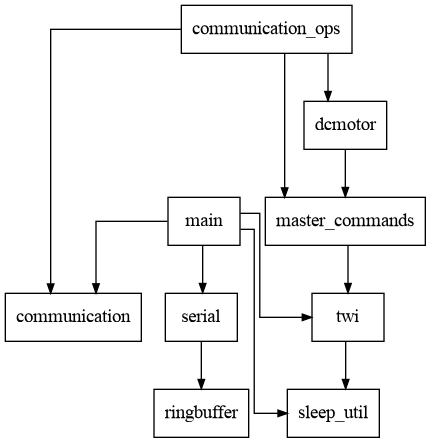
\includegraphics[scale=0.5]{master-deps}
  \caption{Master controller modules dependency graph}
  \label{img:master-deps-graph}
\end{centering}
\end{figure}

\subsection{Circuit schematics}
The complete circuit schematics for the master controller and all its
components is shown in figure \ref{img:master-sch}.
\begin{figure}[hbp]
\begin{centering}
  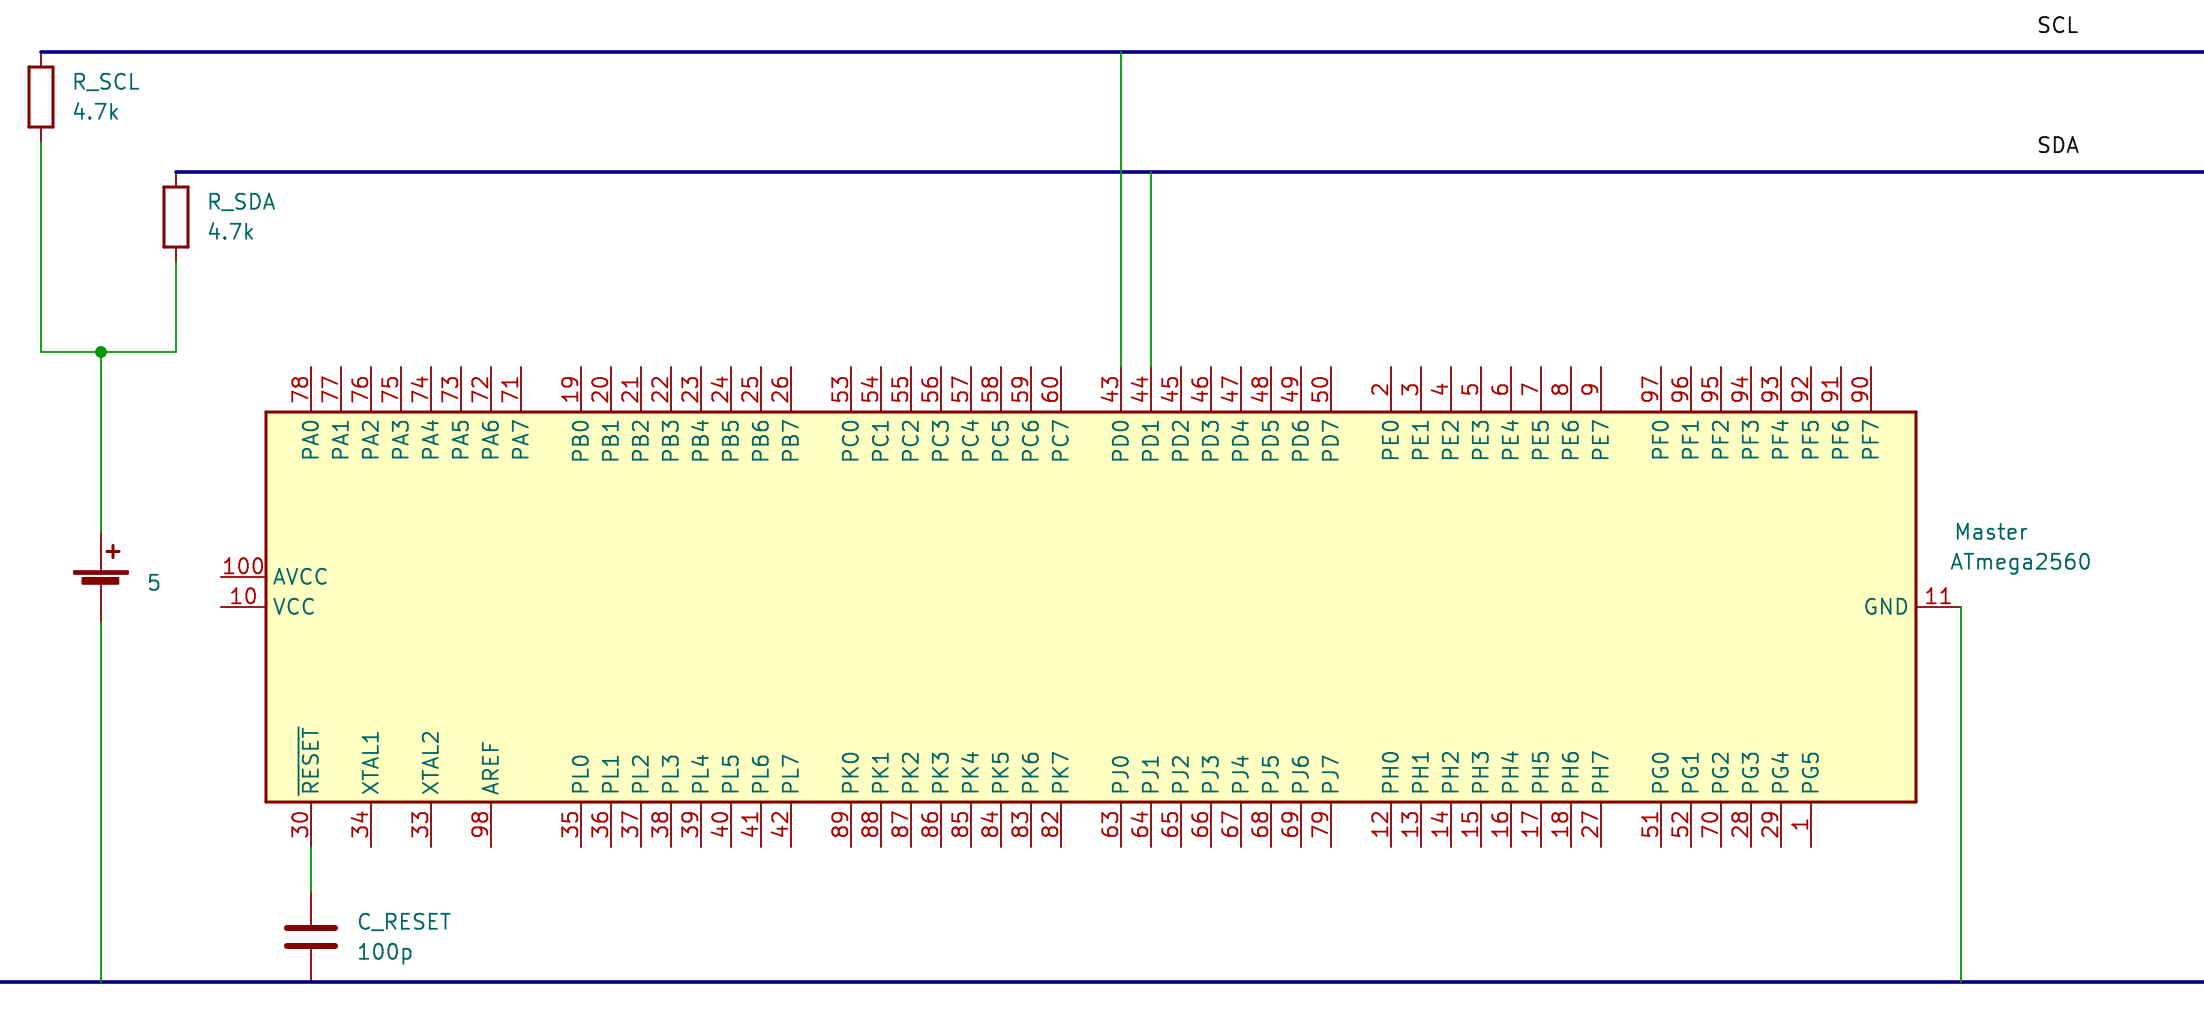
\includegraphics{master-schematics}
  \caption{Master controller schematics}
  \label{img:master-sch}
\end{centering}
\end{figure}

\subsection{Wiring}
The wiring correspondence for the master controller MCU is shown in table
\ref{tab:master-wiring}.
\begin{table}[hb]
  \begin{tabularx}{\textwidth}{c l X}
    \toprule
    Board pin & MCU pin & Description \\
    \midrule
    D20   & 44/PD1/SDA & I2C data bus \\
    D21   & 43/PD0/SCL & I2C clock bus \\
    RESET & RESET      & On-board MCU reset pin \\
    \bottomrule
  \end{tabularx}
  \caption{Master controller wiring}
  \label{tab:master-wiring}
\end{table}
